% Options for packages loaded elsewhere
% Options for packages loaded elsewhere
\PassOptionsToPackage{unicode}{hyperref}
\PassOptionsToPackage{hyphens}{url}
\PassOptionsToPackage{dvipsnames,svgnames,x11names}{xcolor}
%
\documentclass[
]{article}
\usepackage{xcolor}
\usepackage{amsmath,amssymb}
\setcounter{secnumdepth}{5}
\usepackage{iftex}
\ifPDFTeX
  \usepackage[T1]{fontenc}
  \usepackage[utf8]{inputenc}
  \usepackage{textcomp} % provide euro and other symbols
\else % if luatex or xetex
  \usepackage{unicode-math} % this also loads fontspec
  \defaultfontfeatures{Scale=MatchLowercase}
  \defaultfontfeatures[\rmfamily]{Ligatures=TeX,Scale=1}
\fi
\usepackage{lmodern}
\ifPDFTeX\else
  % xetex/luatex font selection
\fi
% Use upquote if available, for straight quotes in verbatim environments
\IfFileExists{upquote.sty}{\usepackage{upquote}}{}
\IfFileExists{microtype.sty}{% use microtype if available
  \usepackage[]{microtype}
  \UseMicrotypeSet[protrusion]{basicmath} % disable protrusion for tt fonts
}{}
\makeatletter
\@ifundefined{KOMAClassName}{% if non-KOMA class
  \IfFileExists{parskip.sty}{%
    \usepackage{parskip}
  }{% else
    \setlength{\parindent}{0pt}
    \setlength{\parskip}{6pt plus 2pt minus 1pt}}
}{% if KOMA class
  \KOMAoptions{parskip=half}}
\makeatother
% Make \paragraph and \subparagraph free-standing
\makeatletter
\ifx\paragraph\undefined\else
  \let\oldparagraph\paragraph
  \renewcommand{\paragraph}{
    \@ifstar
      \xxxParagraphStar
      \xxxParagraphNoStar
  }
  \newcommand{\xxxParagraphStar}[1]{\oldparagraph*{#1}\mbox{}}
  \newcommand{\xxxParagraphNoStar}[1]{\oldparagraph{#1}\mbox{}}
\fi
\ifx\subparagraph\undefined\else
  \let\oldsubparagraph\subparagraph
  \renewcommand{\subparagraph}{
    \@ifstar
      \xxxSubParagraphStar
      \xxxSubParagraphNoStar
  }
  \newcommand{\xxxSubParagraphStar}[1]{\oldsubparagraph*{#1}\mbox{}}
  \newcommand{\xxxSubParagraphNoStar}[1]{\oldsubparagraph{#1}\mbox{}}
\fi
\makeatother


\usepackage{longtable,booktabs,array}
\newcounter{none} % for unnumbered tables
\usepackage{calc} % for calculating minipage widths
% Correct order of tables after \paragraph or \subparagraph
\usepackage{etoolbox}
\makeatletter
\patchcmd\longtable{\par}{\if@noskipsec\mbox{}\fi\par}{}{}
\makeatother
% Allow footnotes in longtable head/foot
\IfFileExists{footnotehyper.sty}{\usepackage{footnotehyper}}{\usepackage{footnote}}
\makesavenoteenv{longtable}
\usepackage{graphicx}
\makeatletter
\newsavebox\pandoc@box
\newcommand*\pandocbounded[1]{% scales image to fit in text height/width
  \sbox\pandoc@box{#1}%
  \Gscale@div\@tempa{\textheight}{\dimexpr\ht\pandoc@box+\dp\pandoc@box\relax}%
  \Gscale@div\@tempb{\linewidth}{\wd\pandoc@box}%
  \ifdim\@tempb\p@<\@tempa\p@\let\@tempa\@tempb\fi% select the smaller of both
  \ifdim\@tempa\p@<\p@\scalebox{\@tempa}{\usebox\pandoc@box}%
  \else\usebox{\pandoc@box}%
  \fi%
}
% Set default figure placement to htbp
\def\fps@figure{htbp}
\makeatother





\setlength{\emergencystretch}{3em} % prevent overfull lines

\providecommand{\tightlist}{%
  \setlength{\itemsep}{0pt}\setlength{\parskip}{0pt}}



 
\usepackage[]{natbib}
\bibliographystyle{plainnat}


\usepackage{iclr2026_conference}
\iclrfinalcopy
\usepackage[hidelinks]{hyperref}
\AtBeginDocument{\author{Divyam Jain\\Technical University of Hamburg (TUHH), Hamburg, Germany\\\texttt{divyam.jain@tuhh.de}}}
\makeatletter
\@ifpackageloaded{caption}{}{\usepackage{caption}}
\AtBeginDocument{%
\ifdefined\contentsname
  \renewcommand*\contentsname{Table of contents}
\else
  \newcommand\contentsname{Table of contents}
\fi
\ifdefined\listfigurename
  \renewcommand*\listfigurename{List of Figures}
\else
  \newcommand\listfigurename{List of Figures}
\fi
\ifdefined\listtablename
  \renewcommand*\listtablename{List of Tables}
\else
  \newcommand\listtablename{List of Tables}
\fi
\ifdefined\figurename
  \renewcommand*\figurename{Figure}
\else
  \newcommand\figurename{Figure}
\fi
\ifdefined\tablename
  \renewcommand*\tablename{Table}
\else
  \newcommand\tablename{Table}
\fi
}
\@ifpackageloaded{float}{}{\usepackage{float}}
\floatstyle{ruled}
\@ifundefined{c@chapter}{\newfloat{codelisting}{h}{lop}}{\newfloat{codelisting}{h}{lop}[chapter]}
\floatname{codelisting}{Listing}
\newcommand*\listoflistings{\listof{codelisting}{List of Listings}}
\makeatother
\makeatletter
\makeatother
\makeatletter
\@ifpackageloaded{caption}{}{\usepackage{caption}}
\@ifpackageloaded{subcaption}{}{\usepackage{subcaption}}
\makeatother
\usepackage{bookmark}
\IfFileExists{xurl.sty}{\usepackage{xurl}}{} % add URL line breaks if available
\urlstyle{same}
\hypersetup{
  pdftitle={Integrating Text-Based Problem Descriptions with Data-driven Partial Differential Equation Solver},
  pdfauthor={Divyam Jain},
  colorlinks=true,
  linkcolor={blue},
  filecolor={Maroon},
  citecolor={Blue},
  urlcolor={Blue},
  pdfcreator={LaTeX via pandoc}}


\title{Integrating Text-Based Problem Descriptions with Data-driven
Partial Differential Equation Solver}
\author{Divyam Jain}
\date{2026-04-20}
\begin{document}
\maketitle
\begin{abstract}
Data-driven Partial Differential Equation (PDE) surrogate models can be
fast and effective, but they often struggle to generalize beyond the
training distribution. This work studies whether natural language
descriptions of physical systems can provide useful high-level context
for improving such generalization. We extend a U-shaped Neural Network
(UNet)-based surrogate model by conditioning it on text embeddings
derived from structured PDE descriptions, and we compare this approach
against an unconditioned UNet and transformer-based Axial Vision
Transformer (AViT) baselines.

Experiments train on turbulent radiative layer and active matter
datasets and evaluate out-of-distribution performance on Helmholtz
staircase. Across rollout-based metrics, the baseline UNet remains the
strongest model, while the conditioned UNet does not consistently
improve accuracy and the transformer baseline performs worse. These
results suggest that simple text conditioning is not enough to improve
out-of-distribution (OOD) generalization in this setting, and that the
success of multimodal PDE modeling depends strongly on how semantic
information is integrated into the architecture.
\end{abstract}


\section{Introduction}\label{introduction}

Partial differential equations (PDEs) underpin many physical,
biological, and engineering models, but solving them accurately at scale
remains computationally expensive. Classical numerical methods are
reliable, yet they often require careful problem-specific design and
become increasingly costly for high-resolution or many-query settings.
This has motivated the use of data-driven surrogate models that learn to
predict PDE dynamics directly from simulation data.

Recent deep learning models have shown that surrogate PDE solvers can be
both accurate and efficient, especially on structured grid data. At the
same time, their performance often depends strongly on the training
distribution. Most models operate only on numerical states and are asked
to infer all relevant physical structure from those states alone, which
makes out-of-distribution (OOD) generalization difficult when the
governing regime, boundary conditions, or equation family changes.

Natural language descriptions offer a different source of information.
PDE systems are often accompanied by structured textual knowledge about
equations, boundary conditions, coefficients, and qualitative behavior.
Modern large language models (LLMs) can embed this information into
dense vectors, making it possible to condition numerical surrogate
models on compact semantic context instead of relying only on raw state
trajectories.

This work studies whether such text-based conditioning improves PDE
surrogate modeling. We extend a UNet-based architecture with text
embeddings derived from structured PDE descriptions and compare it
against an unconditioned UNet and transformer-based Axial Vision
Transformer (AViT) baselines. The models are trained on turbulent
radiative layer and active matter data and evaluated on the OOD
Helmholtz staircase dataset using rollout-based error metrics.

Our main finding is negative but informative: simple text conditioning
does not improve performance in this setting. The baseline UNet remains
strongest, the conditioned UNet does not consistently outperform it, and
the reported AViT runs lag behind both. These results suggest that
multimodal PDE modeling is less about adding another modality and more
about aligning that modality with the inductive bias of the solver.

The main contributions of this paper are:

\begin{enumerate}
\def\labelenumi{\arabic{enumi}.}
\tightlist
\item
  We implement a text-conditioned UNet surrogate model that injects PDE
  descriptions, encoded with a frozen sentence embedding model, into a
  grid-based forecasting pipeline.
\item
  We evaluate this conditioned model against an unconditioned UNet
  baseline and representative AViT transformer runs in a multi-dataset
  setting with explicit OOD testing on Helmholtz staircase.
\item
  We show that lightweight text conditioning does not improve OOD
  rollout performance in this setup, and we use that negative result to
  argue that solver inductive bias and fusion design matter more than
  simply adding semantic metadata.
\end{enumerate}

\section{Problem Setting and
Motivation}\label{problem-setting-and-motivation}

This section introduces the problem setting and the architectural
motivation for text conditioning. The next section focuses specifically
on prior literature and how this project is positioned relative to it.

\subsection{Partial Differential Equations in Scientific
Modeling}\label{partial-differential-equations-in-scientific-modeling}

Partial differential equations (PDEs) describe how physical quantities
such as temperature, velocity, pressure, and concentration evolve over
space and time. Classical examples include diffusion, wave propagation,
and fluid flow. In this work, one benchmark system is the
two-dimensional turbulent radiative layer, whose governing equations are
shown in \autoref{eq:turbulent_radiative}.

\begin{equation}
\label{eq:turbulent_radiative}
\begin{array}{rcl}
\frac{\partial \rho}{\partial t} + \nabla \cdot (\rho \mathbf{v}) & = & 0, \\
\frac{\partial (\rho \mathbf{v})}{\partial t} + \nabla \cdot (\rho \mathbf{v} \otimes \mathbf{v} + P\mathbf{I}) & = & \mathbf{0}, \\
\frac{\partial E}{\partial t} + \nabla \cdot ((E + P)\mathbf{v}) & = & -\frac{E}{t_{\mathrm{cool}}}, \\[0.3em]
\multicolumn{3}{c}{E = \frac{P}{\gamma - 1}, \qquad \gamma = \frac{5}{3}.}
\end{array}
\end{equation}

Here \(\rho\) denotes density, \(\mathbf{v}\) velocity, \(P\) pressure,
\(E\) internal energy density, \(\mathbf{I}\) the identity tensor, and
\(\otimes\) the outer product.

Analytical solutions exist only for a limited class of problems, so most
realistic PDEs are solved numerically using methods such as finite
differences, finite elements, or spectral discretizations. These methods
are accurate and physically grounded, but they are also computationally
expensive and often require substantial problem-specific design.
\autoref{fig:active_matter_turbulent} shows example fields from the
active matter and turbulent radiative layer datasets used in this study.

\begin{figure}[h]
\centering
\caption{Example fields from the datasets used in this study: (a) active matter and (b) turbulent radiative layer.}
\label{fig:active_matter_turbulent}
\begin{minipage}{0.48\textwidth}
\centering

\includegraphics[width=\textwidth]{figures/active_matter_turbulent.png}
\end{minipage}
\hfill
\begin{minipage}{0.34\textwidth}
\centering

\includegraphics[width=\textwidth]{figures/concentration_notnormalized.png}
\end{minipage}
\end{figure}

\subsection{Data-Driven Surrogates and
Generalization}\label{data-driven-surrogates-and-generalization}

The rise of machine learning has introduced surrogate models that learn
mappings from input states to future system behavior directly from
simulation data. Once trained, these models can produce predictions much
faster than repeatedly running a full numerical solver. Convolutional
architectures such as UNets are especially useful for grid-based PDE
data because their local connectivity and weight sharing align with
spatially structured fields.

However, data-driven PDE solvers still depend on representative training
data. Generating this data often requires computationally expensive
simulations, and learned models may overfit to the regimes included in
those simulations. This makes generalization a central challenge,
especially when a model is evaluated under new parameters, boundary
conditions, or governing equations.

Generalization is a key requirement for practical PDE solvers. In many
applications, a model must operate under conditions that differ from
those seen during training, including new initial conditions,
parameters, boundary conditions, or even governing equations. Such
scenarios are commonly referred to as OOD settings.

Data-driven models often perform well in-distribution but degrade
sharply in OOD settings because they learn correlations from the
training data rather than broadly transferable physical structure. A
model trained on one coefficient range or one type of boundary condition
may therefore fail when those assumptions change. This motivates the
search for additional signals that can guide models toward more robust
behavior.

\subsection{Architecture, Inductive Bias, and Text
Conditioning}\label{architecture-inductive-bias-and-text-conditioning}

Inductive bias refers to the assumptions a model makes about the
structure of the data. In the context of PDEs, different architectures
encode different inductive biases that influence their performance.
Convolutional neural networks (CNNs), for instance, assume local spatial
correlations and translation invariance, which align well with many
physical systems. This makes them particularly effective for grid-based
PDE problems.

On the other hand, transformer-based models rely on attention mechanisms
that capture global dependencies. While this can be advantageous for
certain tasks, it may not always align with the local nature of
differential operators in PDEs. Additionally, transformers typically
require larger datasets and longer training times to achieve comparable
performance.

Multimodal learning combines different sources of information to improve
prediction. In PDE modeling, text can provide structured context about
the governing equation, boundary conditions, and qualitative system
behavior. In this study, text is treated as metadata that complements
numerical input rather than replaces it.

The motivation for this work arises from the intersection of these
observations. Data-driven PDE solvers still struggle with OOD behavior,
and textual descriptions provide rich contextual information that is
currently underused in scientific machine learning. This work therefore
tests whether text-based conditioning can improve OOD behavior in PDE
surrogate models. At the same time, it treats multimodal learning as an
architectural question rather than a guaranteed benefit: if text is
useful, the model still needs a way to fuse semantic and
spatial-temporal information effectively. Comparing convolutional and
transformer-based models therefore helps clarify whether performance
depends more on additional context or on the underlying inductive bias
of the solver.

\section{Related Work}\label{related-work}

\subsection{Classical, Neural, and Operator-Based PDE
Solvers}\label{classical-neural-and-operator-based-pde-solvers}

Classical PDE solvers such as finite difference, finite element, and
spectral methods remain the standard tools because they are accurate and
physically grounded. Their drawback is cost: they can be slow to run
repeatedly and often need careful hand-designed discretizations for each
new problem.

Neural surrogate models try to learn a shortcut. Instead of solving the
equations from scratch every time, they learn from many examples and
then predict the next state quickly. Early neural approaches such as
physics-informed neural networks (PINNs) add the PDE itself to the loss
so the network is punished when it violates known physics
\citep{raissi2019pinns, pinnsagent}. Operator-learning methods such as
DeepONet and Fourier Neural Operator (FNO) go one step further: rather
than memorizing one trajectory, they learn a mapping from one function
to another \citep{deeponet2021, fno2021}. In simple terms, they try to
learn the rule of the game, not just one game result.

Another closely related idea is message passing on spatial grids or
graphs. Message Passing Neural PDE Solvers (MPP) learn how nearby
spatial locations exchange information over time \citep{mpp}. This is a
natural fit for PDEs because many physical laws are local: what happens
at one point usually depends most strongly on its neighbors. These
families of models are fast after training, but they can still struggle
when the test problem looks meaningfully different from the training
problems.

\subsection{Transformer-Based PDE
Solvers}\label{transformer-based-pde-solvers}

Transformer-based PDE models ask whether a more flexible architecture
can generalize across many physical systems by combining field
information with more structured global context.

Unisolver is a representative example \citep{unisolver}. It conditions
the model on structured PDE ingredients such as equation terms,
coefficients, and boundary conditions. This is important because two
systems can exhibit similar instantaneous states while still evolving
differently under distinct governing equations or boundary constraints.
By incorporating these structured descriptors explicitly, the model is
better positioned to separate visual similarity from physical
equivalence.

A second direction is large-scale pretraining across many physical
systems. Multi-physics pretraining (MPP) aims to expose a model to
diverse simulation families so that it learns reusable physical patterns
before being adapted to a specific task \citep{mpp}. This is attractive
because PDE generalization usually fails when a model only knows one
narrow regime. However, transformer-style models also bring costs: they
often need more data, more compute, and stronger regularization than
convolutional baselines, and they may be less naturally aligned with
strongly local operators.

\subsection{Text-Conditioned and Multimodal PDE
Models}\label{text-conditioned-and-multimodal-pde-models}

Recent work has started to add language directly to PDE modeling.
Lorsung and Barati Farimani study whether pretrained language embeddings
can help surrogate models when the text describes the system being
solved \citep{lorsung2024}. Text2PDE explores a more generative setup,
where language is used to guide physics simulation through latent
diffusion \citep{text2pde}. In both cases, the central idea is simple: a
short text description can summarize things that may be hard to infer
from raw fields alone, such as the type of equation, the forcing, or the
boundary behavior.

This is promising, but it is not automatic. A text embedding is only
useful if the numerical model knows how to use it. If the fusion
mechanism is weak, the text becomes just another vector attached to the
input and may be ignored. That is why multimodal PDE learning is still
an open problem rather than a solved recipe.

\subsection{Symbolic, Hybrid, and LLM-Guided
Directions}\label{symbolic-hybrid-and-llm-guided-directions}

Another branch of the literature uses language-model-style systems more
directly for symbolic reasoning. CodePDE, for example, frames PDE
solving as an inference and generation problem in which the model helps
construct solver logic rather than only forecasting states
\citep{codepde2025}. Hybrid work in this area combines neural
prediction, symbolic structure, and physics constraints to improve
interpretability or automation.

These methods are exciting, but they answer a somewhat different
question from the one studied here. They focus on generating solver
procedures or symbolic forms, whereas this report focuses on rollout
prediction for grid-based surrogate models.

\subsection{Research Gap and
Positioning}\label{research-gap-and-positioning}

The literature now covers strong convolutional surrogates, operator
learners, transformer-based universal solvers, and early
text-conditioned systems. The missing piece is still the interaction
between semantic conditioning and architectural bias. We do not yet know
whether a simple text vector helps a local convolutional solver
generalize better, or whether text only becomes useful when paired with
richer fusion mechanisms such as cross-attention.

This report targets that gap. It keeps the conditioning mechanism
intentionally lightweight, applies it to a UNet-style surrogate, and
compares the result against both an unconditioned UNet and
representative AViT transformer runs. That makes the contribution
narrower than a foundation-model paper, but clearer: it isolates whether
simple text conditioning helps OOD PDE rollout prediction in a practical
grid-based setting.

\section{Methodology}\label{methodology}

\subsection{Problem Formulation}\label{problem-formulation}

We consider the problem of learning a data-driven surrogate model for
solving PDEs. Let the physical system be described by a PDE of the form:

\begin{equation}
\mathcal{F}(u, \nabla u, \nabla^2 u, x, t; \theta) = 0
\end{equation}

where \(u(x,t)\) represents the system state defined over spatial domain
\(x \in \Omega\) and time \(t \in \mathbb{R}^+\), and \(\theta\) denotes
system-specific parameters such as coefficients and boundary conditions.

The goal is to learn a parameterized evolution map that approximates
one-step dynamics:

\begin{equation}
\hat{u}_{t+1} = f_\phi(u_{t-T_i+1:t}, c)
\end{equation}

where: - \(u_{t-T_i+1:t}\) denotes the sequence of \(T_i\) input
timesteps, - \(c\) represents the projected text-conditioning vector, -
\(f_\phi\) is a neural network parameterized by \(\phi\).

\subsection{Data Representation}\label{data-representation}

Each PDE state is represented as a multi-channel tensor:
\(u_t \in \mathbb{R}^{C \times H \times W}\), where \(C\) denotes the
number of physical variables and \(H, W\) denote the spatial resolution.

The input to the model is constructed by stacking past timesteps along
the channel dimension:

\begin{equation}
X_t = [u_{t-T_i+1}, \ldots, u_t] \in \mathbb{R}^{(T_i C) \times H \times W}.
\end{equation}

The target output is:

\begin{equation}
Y_t = [u_{t+1}, \ldots, u_{t+T_o}] \in \mathbb{R}^{(T_o C) \times H \times W}.
\end{equation}

\subsection{Text-Based Conditioning}\label{text-based-conditioning}

To incorporate high-level physical context, we use natural language
descriptions of PDE systems. Each description includes:

\begin{itemize}
\tightlist
\item
  Governing equations
\item
  Boundary conditions
\item
  Operator coefficients
\item
  Qualitative system behavior
\end{itemize}

These descriptions are processed using the frozen SentenceTransformer
model \texttt{sentence-transformers/all-MiniLM-L6-v2}. Let \(s\) denote
the text description and \(g_{\mathrm{MiniLM}}\) denote this frozen
encoder. The resulting embeddings are cached in
\texttt{pde\_text\_embeddings.pt} and reused during training:

\begin{equation}
e = g_{\mathrm{MiniLM}}(s), \qquad e \in \mathbb{R}^{384}.
\end{equation}

The embedding is then projected into a conditioning vector using a
feedforward network:

\begin{equation}
 c = W_2 \sigma(W_1 e + b_1) + b_2
\end{equation}

where:

\begin{itemize}
\tightlist
\item
  \(\sigma\) is the SiLU activation function,
\item
  \(W_1 \in \mathbb{R}^{128 \times 384}\) and
  \(W_2 \in \mathbb{R}^{16 \times 128}\) are learnable parameters,
\item
  \(c \in \mathbb{R}^{16}\) is the projected conditioning vector.
\end{itemize}

\subsection{Text Conditioning
Descriptions}\label{text-conditioning-descriptions}

The conditioning descriptions used in this work follow a compact
four-layer schema before embedding with
\texttt{sentence-transformers/all-MiniLM-L6-v2}:

\begin{enumerate}
\def\labelenumi{\arabic{enumi}.}
\tightlist
\item
  Basic description: outlines the equation type and core physical
  properties.
\item
  Boundary conditions: adds constraint information at the domain
  boundaries.
\item
  Operator coefficients: specifies the numerical parameters that appear
  in the PDE.
\item
  Qualitative behavior: captures intuitive dynamics that may not be
  written explicitly in the equation.
\end{enumerate}

\textbf{Turbulent radiative layer.} Turbulent radiative layer in two
spatial dimensions governed by compressible Navier--Stokes equations
coupled with thermal energy transport. The system includes nonlinear
advection, viscous diffusion, and buoyancy forcing driven by vertical
temperature gradients. Lower boundary injects heat, upper boundary
removes heat through radiative cooling, horizontal boundaries are
periodic. Flow regime is convection driven and turbulence dominated. The
solution develops multi-scale vortices, thermal plumes, and chaotic
velocity structures. The predicted state should exhibit intermittent
turbulent mixing and filamentary temperature fields.

\textbf{Active matter.} Two-dimensional active matter system governed by
nonlinear hydrodynamic equations with self-propulsion forcing and
diffusive regularization. The velocity field includes advective
transport and active energy injection at small scales. Periodic boundary
conditions in both spatial directions. The system is far from
equilibrium and activity dominated. The solution develops spontaneous
vortices, traveling bands, and long-range collective motion. The
predicted state should exhibit coherent swirling structures and
dynamically forming clusters.

\subsection{UNet-Based Architecture}\label{unet-based-architecture}

\begin{figure}[h!]
\centering
\caption{UNet architecture used in this work.}
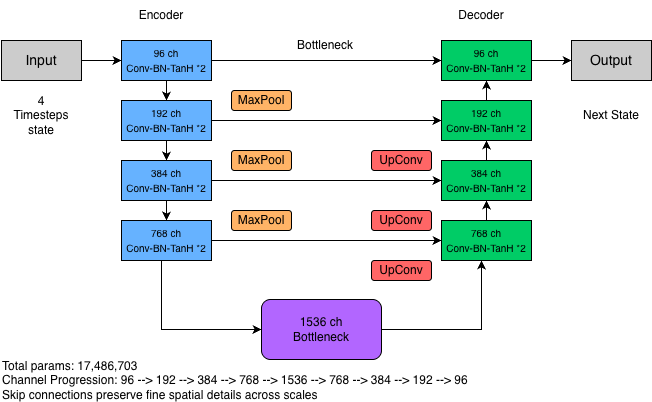
\includegraphics[width=0.9\textwidth]{figures/unet_diagram.png}
\label{fig:unet}
\end{figure}

The backbone of our model is a UNet architecture, which consists of an
encoder--decoder structure with skip connections as shown in
\autoref{fig:unet}.

\subsubsection{Encoder}\label{encoder}

The encoder progressively extracts hierarchical features:

\begin{equation}
h_1 = B_1(X_t), \qquad h_l = B_l(\operatorname{Pool}(h_{l-1})), \quad l = 2,\ldots,4.
\end{equation}

Each block consists of two repeated convolutional stages with batch
normalization and Tanh activations.

The spatial resolution is reduced using max pooling, while the number of
channels increases:

\begin{equation}
48 \rightarrow 96 \rightarrow 192 \rightarrow 384 \rightarrow 768
\end{equation}

\subsubsection{Bottleneck}\label{bottleneck}

At the lowest resolution, the model captures global context:

\begin{equation}
h_{\mathrm{b}} = B_{\mathrm{b}}(\operatorname{Pool}(h_4))
\end{equation}

\subsubsection{Decoder}\label{decoder}

The decoder reconstructs the output through upsampling:

\begin{equation}
\tilde{h}_l = D_l(\operatorname{Concat}_{\mathrm{ch}}(\operatorname{Up}(\tilde{h}_{l+1}), h_l)), \quad l = 4,\ldots,1.
\end{equation}

where: - \(\operatorname{Up}(\cdot)\) denotes transposed-convolution
upsampling, - \(h_l\) denotes the skip connection from the encoder.

\subsection{Conditioning Integration}\label{conditioning-integration}

The conditioning vector \(c\) is integrated into the model by augmenting
the input representation:

\begin{equation}
X'_t = \operatorname{Concat}_{\mathrm{ch}}(X_t, c^\uparrow), \qquad c^\uparrow \in \mathbb{R}^{16 \times H \times W}.
\end{equation}

where \(c^\uparrow\) is a spatially broadcasted version of the
conditioning vector.

This allows the model to adapt its predictions based on textual context.

\subsection{Experimental Pipeline}\label{experimental-pipeline}

The full experimental pipeline used in this project is summarized in
\autoref{fig:experimental_pipeline}. A structured PDE description is
first embedded with a frozen text encoder, while the numerical branch
receives four input timesteps of multi-channel PDE fields. The
conditioned UNet concatenates both sources of information to predict the
next state, and performance is then evaluated through autoregressive
rollout on an OOD benchmark.

\begin{figure}[h!]
\centering
\caption{Experimental pipeline used in this project. The model combines structured PDE descriptions with numerical field histories, predicts the next timestep, and is evaluated through OOD rollout.}
\label{fig:experimental_pipeline}
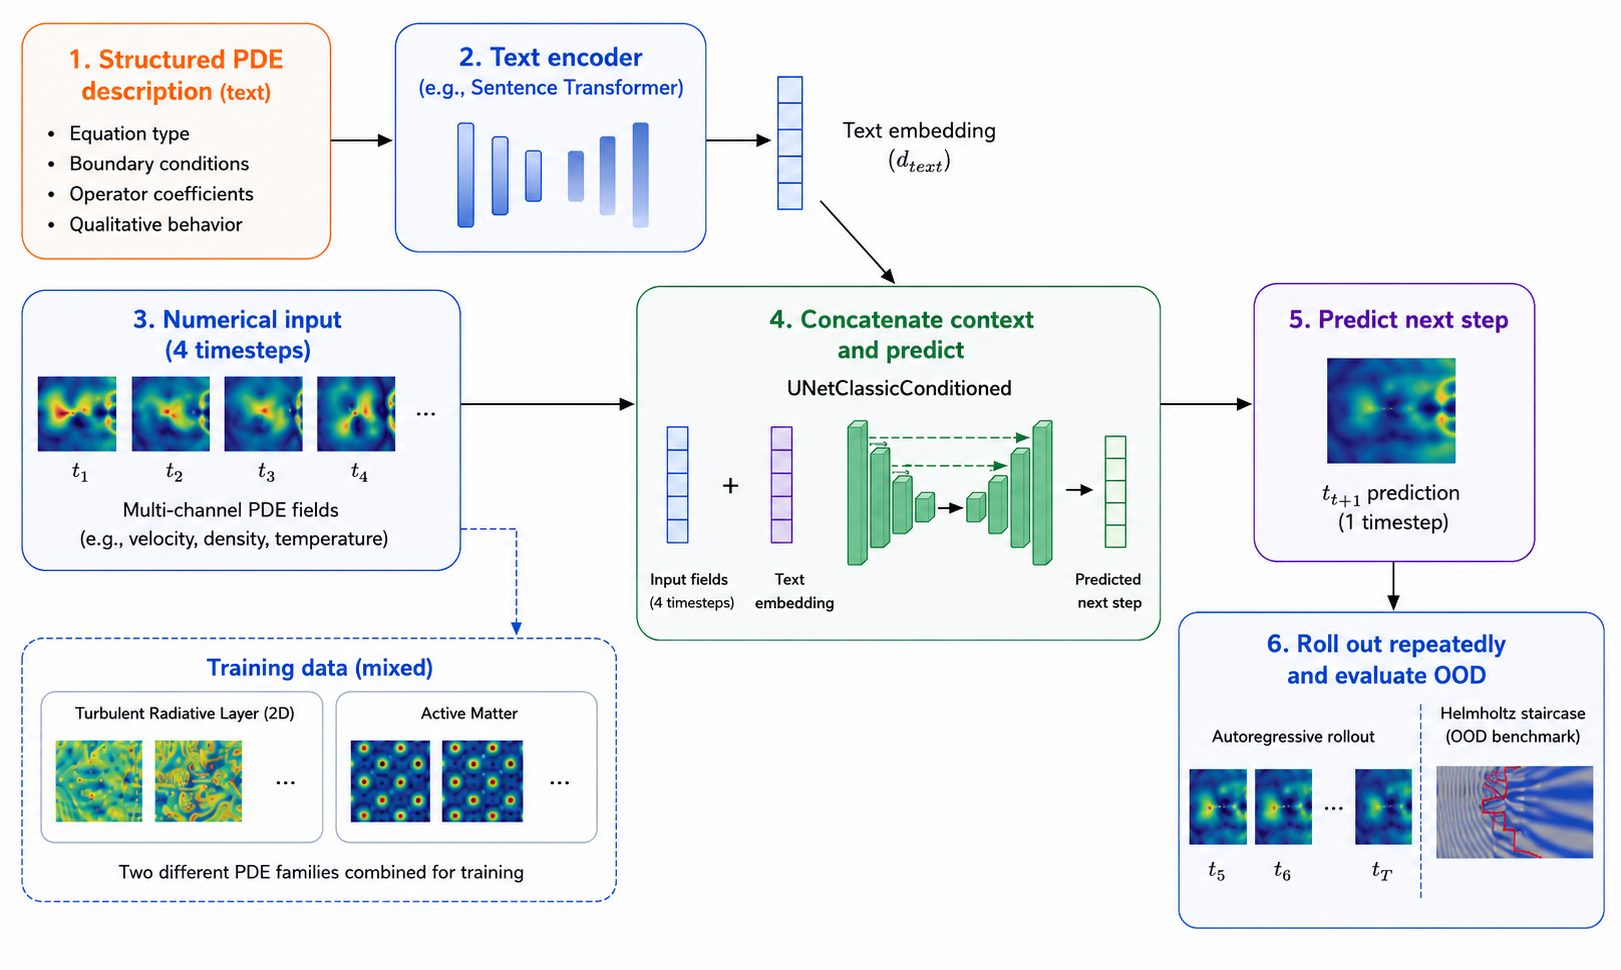
\includegraphics[width=\textwidth]{figures/experimental_pipeline.png}
\end{figure}

\subsection{Training Objective}\label{training-objective}

The model is trained using supervised learning with a mean squared error
(MSE) loss:

\begin{equation}
L_{\mathrm{MSE}} = \frac{1}{N} \sum_{i=1}^{N} \|\hat{u}_i - u_i\|_2^2
\end{equation}

To evaluate robustness, we also consider rollout loss over multiple
timesteps:

\begin{equation}
L_{\mathrm{rollout}} = \frac{1}{T_r} \sum_{\tau=1}^{T_r} L_{\mathrm{MSE}}(\hat{u}_{t+\tau}, u_{t+\tau})
\end{equation}

\subsection{Training Procedure}\label{training-procedure}

At each iteration, the model samples an input-target pair, computes the
text embedding and projected conditioning vector, predicts the next
state, and updates parameters using the training loss.

\subsection{Evaluation Protocol}\label{evaluation-protocol}

We evaluate models using multi-step rollout:

\begin{itemize}
\tightlist
\item
  Predict one step ahead
\item
  Feed prediction back as input
\item
  Repeat for multiple timesteps
\end{itemize}

Metrics used:

\begin{itemize}
\tightlist
\item
  Mean Squared Error (MSE)
\item
  Root Mean Squared Error (RMSE)
\item
  Maximum error (\(L_\infty\))
\end{itemize}

This setup tests both short-term accuracy and long-term stability.

\subsection{Baselines}\label{baselines}

We compare:

\begin{itemize}
\tightlist
\item
  UNetClassic (unconditioned baseline)
\item
  UNetClassicConditioned (text-conditioned baseline)
\item
  Axial Vision Transformer (AViT) (transformer baseline)
\end{itemize}

\subsection{Methodological Design
Choices}\label{methodological-design-choices}

Overall, the methodology combines spatial modeling via a UNet backbone,
temporal modeling via stacked input frames, and semantic conditioning
via text embeddings. The central design question is whether this
relatively simple fusion strategy is strong enough to improve OOD PDE
surrogate modeling without disrupting the inductive bias that makes
convolutional models effective on grid-structured physical fields.

\section{Experiments and Results}\label{experiments-and-results}

\subsection{Model Implementation}\label{model-implementation}

The models were implemented in the project repository using a
GPU-accelerated deep learning pipeline. The UNet baseline and the
conditioned UNet follow the methodology described above; in practice,
the conditioned variant adds the frozen
\texttt{sentence-transformers/all-MiniLM-L6-v2} embedding pathway and
projects text features from
\(\mathbb{R}^{384} \rightarrow \mathbb{R}^{128} \rightarrow \mathbb{R}^{16}\)
before broadcasting them across the spatial grid.

The repository currently exposes a single AViT configuration without a
separate text-conditioning path. For that reason, the AViT results
reported below should be interpreted as representative
transformer-baseline runs rather than as a matched
conditioned-versus-unconditioned AViT comparison.

\subsection{Dataset and Preprocessing}\label{dataset-and-preprocessing}

The experiments were conducted on multiple PDE datasets:

\begin{itemize}
\tightlist
\item
  Training datasets:

  \begin{itemize}
  \tightlist
  \item
    Turbulent Radiative Layer (2D)
  \item
    Active Matter
  \end{itemize}
\item
  Validation datasets:

  \begin{itemize}
  \tightlist
  \item
    Turbulent Radiative Layer (2D)
  \item
    Active Matter
  \end{itemize}
\item
  Test dataset (OOD):

  \begin{itemize}
  \tightlist
  \item
    Helmholtz Staircase
  \end{itemize}
\end{itemize}

Each dataset consists of spatiotemporal simulations represented as
multi-channel tensors. The spatial resolution is fixed at
\(128 \times 384\), and temporal sequences are constructed using:

\begin{itemize}
\tightlist
\item
  Input timesteps: 4
\item
  Output timesteps: 1
\end{itemize}

Input sequences are formed by stacking consecutive frames along the
channel dimension. In the multi-dataset setting, all fields are resized
to a common \(128 \times 384\) grid and remapped into a shared channel
schema so that models can process turbulent radiative layer, active
matter, and Helmholtz staircase data with the same input and output
dimensionality. All data is normalized to ensure stable training.

\subsection{Training Configuration}\label{training-configuration}

The models were trained using the following setup:

\begin{itemize}
\tightlist
\item
  Optimizer: AdamW
\item
  Learning rate: \(10^{-2}\)
\item
  Weight decay: \(10^{-4}\)
\item
  Learning rate scheduler: Linear warmup followed by cosine annealing
\item
  Loss function: Mean Squared Error (MSE)
\item
  Evaluation: Multi-step rollout
\item
  Number of epochs: 20
\item
  Batch size: 8
\end{itemize}

Training was performed for a fixed number of epochs, and performance was
evaluated on both in-distribution and out-of-distribution datasets. The
in-distribution (ID) validation set uses the same PDE families as
training, while the Helmholtz staircase test set is reserved for OOD
evaluation. The headline values in \autoref{tbl-rollout_loss} and
\autoref{tbl-rollout_metrics} are taken from a consistent set of saved
experiment summaries: \texttt{UNetClassic-0.01/6},
\texttt{UNetClassicConditioned-0.01/5}, and two representative
\texttt{AViT-0.01} runs (\texttt{/9} and \texttt{/8}) from the
multi-dataset experiment folder.

\subsection{Overall Performance}\label{overall-performance}

Because OOD generalization is the main research question in this work,
\autoref{tbl-rollout_loss} explicitly separates in-distribution and
out-of-distribution results. The table compares validation loss on the
in-distribution validation set with rollout test loss on the Helmholtz
staircase OOD test set, and the final column reports the corresponding
generalization gap.

\begin{table}

\caption{\label{tbl-rollout_loss}In-distribution and OOD performance.}

\centering{

\centering


\begin{tabular}{l c c c}
\toprule
Model & ID Val. Loss & OOD Test Loss & Gen. Gap \\
\midrule
UNetClassic (baseline) & 0.00948 & 0.13623 & 0.12675 \\
UNetClassicConditioned & 0.00982 & 0.13802 & 0.12820 \\
AViT (representative run A) & 0.01134 & 0.41496 & 0.40362 \\
AViT (representative run B) & 0.01146 & 0.48020 & 0.46873 \\
\bottomrule
\end{tabular}

}

\end{table}%

All models achieve relatively low in-distribution validation loss, but
performance degrades substantially on the OOD Helmholtz staircase test
set. The baseline UNet retains the smallest degradation, while the
conditioned UNet and the two representative AViT runs exhibit markedly
larger generalization gaps.

\begin{figure}[h]
\centering
\caption{Rollout loss on the Helmholtz staircase OOD evaluation.}
\label{fig:rollout}
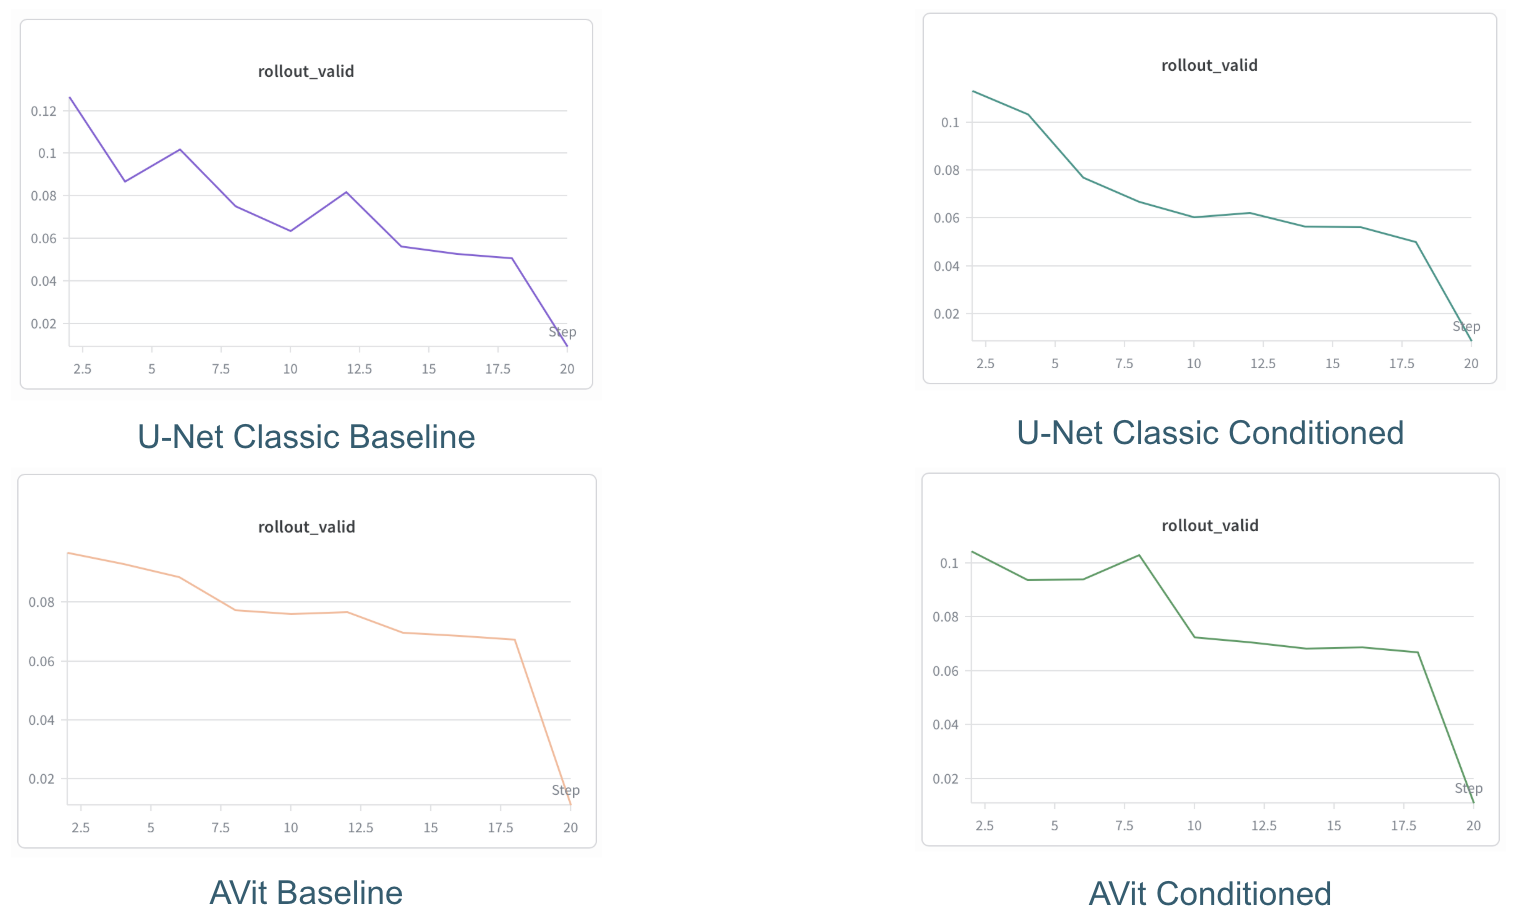
\includegraphics[width=0.9\textwidth]{figures/rollout_loss.png}
\end{figure}

As shown in \autoref{fig:rollout}, the rollout loss curve highlights
that the baseline UNetClassic model accumulates error more slowly than
both the conditioned UNet and the reported AViT runs. This visual trend
supports the numerical results in \autoref{tbl-rollout_metrics}, which
report OOD-only rollout metrics on the Helmholtz staircase test set.

\begin{table}

\caption{\label{tbl-rollout_metrics}OOD rollout metrics on Helmholtz staircase.}

\centering{

\centering


\begin{tabular}{l c c c c}
\toprule
Model & OOD Rollout Test Loss & MSE ($D_{xx}$) & RMSE & $L_\infty$ Error \\
\midrule
UNetClassic (baseline) & 0.13623 & 0.00096 & 0.03091 & 0.18391 \\
UNetClassicConditioned & 0.13802 & 0.00637 & 0.07981 & 0.23783 \\
AViT (representative run A) & 0.41496 & 0.18382 & 0.40078 & 1.48433 \\
AViT (representative run B) & 0.48020 & 0.23509 & 0.45017 & 1.51812 \\
\bottomrule
\end{tabular}

}

\end{table}%

The results for \(T_i=4\) are presented in
\autoref{tbl-rollout_metrics}. The UNetClassic model (without embedding)
achieves the best OOD performance, with the lowest rollout loss and the
most favorable error metrics across all evaluations. The conditioned
variant (UNetClassicConditioned) performs slightly worse, indicating
that text embedding does not improve performance in this setting. The
two representative AViT runs perform substantially worse than the
UNet-based models, with OOD rollout losses between 0.41496 and 0.48020.
This again suggests that architectural suitability matters more than
simply switching to a transformer baseline.

\subsection{Field-wise Error Analysis}\label{field-wise-error-analysis}

A detailed evaluation on individual fields (e.g., \(D_{xx}\)) reveals:

\begin{itemize}
\tightlist
\item
  UNetClassic achieves the lowest error across all metrics
\item
  UNetClassicConditioned shows significant degradation:

  \begin{itemize}
  \tightlist
  \item
    approximately \(6.7\times\) higher MSE
  \item
    approximately \(1.3\times\) higher \(L_\infty\) error
  \end{itemize}
\item
  AViT models exhibit the highest errors across all metrics
\end{itemize}

These results indicate that the baseline model is more effective at
capturing the underlying dynamics.

\subsection{Parameter Norm Analysis}\label{parameter-norm-analysis}

The parameter norms of the representative checkpoints are:

\begin{itemize}
\tightlist
\item
  UNetClassic: \textasciitilde2597
\item
  UNetClassicConditioned: \textasciitilde2924
\item
  AViT: \textasciitilde3850+
\end{itemize}

Larger parameter norms in the AViT checkpoints do not translate into
better OOD performance. This suggests that raw parameter magnitude is
not the limiting factor and again highlights the importance of
architectural suitability.

\subsection{Model Complexity}

To ensure a fair comparison between architectures, we report the total
number of trainable parameters for each model:

\begin{itemize}
    \item UNetClassic: 17,512,623 parameters
    \item UNetClassicConditioned: 17,570,879 parameters
    \item AViT (representative runs A and B): 14,841,856 parameters each
\end{itemize}

The conditioned UNet model introduces a marginal increase in parameters
due to the additional projection layers used for incorporating text
embeddings. The AViT architecture keeps the same parameter count across
the reported runs because the repository currently exposes a single AViT
configuration.

Despite having fewer parameters, AViT models underperform compared to
UNet-based architectures, indicating that performance differences are
primarily driven by architectural inductive bias rather than model size.

\subsection{Effect of Text
Conditioning}\label{effect-of-text-conditioning}

One of the key findings of this work is that text conditioning does not
improve performance in the current setup. While the hypothesis suggested
that textual information could enhance generalization, the experimental
results indicate otherwise.

Several factors contribute to this outcome:

\begin{itemize}
\tightlist
\item
  Redundant information: The multi-dataset training setup already
  encodes dataset identity through channel structure, reducing the need
  for additional conditioning.
\item
  Weak alignment between modalities: The text embeddings may not align
  effectively with the numerical features learned by the UNet.
\item
  Overfitting to conditioning signal: The additional parameters
  introduced by the conditioning module may lead to overfitting without
  improving generalization.
\end{itemize}

These observations suggest that simply adding text embeddings is
insufficient, and more sophisticated integration strategies are
required.

\subsection{Architectural
Considerations}\label{architectural-considerations}

The comparison between UNet and AViT highlights the importance of
inductive bias in model design.

\begin{itemize}
\tightlist
\item
  UNet advantages:

  \begin{itemize}
  \tightlist
  \item
    Strong inductive bias for grid-based data
  \item
    Efficient local feature extraction
  \item
    Multi-scale representation through pooling
  \end{itemize}
\item
  AViT limitations:

  \begin{itemize}
  \tightlist
  \item
    Attention mechanisms are not well-suited for local PDE operators
  \item
    Requires larger datasets and longer training
  \item
    Higher computational complexity
  \end{itemize}
\end{itemize}

As a result, the UNet architecture is better aligned with the structure
of PDE data, leading to superior performance.

\subsection{Generalization and OOD
Performance}\label{generalization-and-ood-performance}

The evaluation on the Helmholtz staircase dataset demonstrates that
generalization remains a challenging problem. While the baseline UNet
performs well, the conditioned model does not show improved OOD
performance.

This gap is also visible when comparing in-distribution and
out-of-distribution losses directly. In one representative run, the
training loss decreases from approximately 1.05 to 0.0069 by epoch 20,
while the validation loss remains low at about 0.0103. In contrast, the
final test loss rises to 0.1398. This indicates that the model fits the
training and validation distributions well, but degrades substantially
on the OOD test setting. Since Helmholtz staircase is used as the OOD
benchmark, this separation between ID and OOD performance should be made
explicit in the interpretation of the results.

This suggests that:

\begin{itemize}
\tightlist
\item
  The conditioning signal is not effectively guiding the model
\item
  The model still relies primarily on learned numerical patterns
\end{itemize}

Improving OOD generalization requires:

\begin{itemize}
\tightlist
\item
  Better fusion mechanisms
\item
  More expressive representations of physical knowledge
\end{itemize}

\subsection{Implications for Multimodal PDE
Modeling}\label{implications-for-multimodal-pde-modeling}

The results of this work provide important insights into multimodal
learning for scientific applications:

\begin{itemize}
\tightlist
\item
  Multimodal inputs can be beneficial, but integration strategy is
  critical
\item
  Architectural alignment is more important than simply increasing model
  complexity
\item
  Text-based conditioning requires careful design to be effective
\end{itemize}

These findings highlight the need for future research in:

\begin{itemize}
\tightlist
\item
  Cross-modal attention mechanisms
\item
  Physics-aware embedding strategies
\item
  Hybrid architectures combining CNNs and transformers
\end{itemize}

\subsection{Discussion}\label{discussion}

The implementation and evaluation together demonstrate that:

\begin{itemize}
\tightlist
\item
  UNet-based models are highly effective for PDE surrogate modeling
\item
  Text conditioning, in its current form, does not improve performance
\item
  Transformer-based models underperform due to architectural mismatch
\end{itemize}

The results emphasize that model design and modality integration are key
factors in developing robust and generalizable PDE solvers.

\section{Limitations}\label{limitations}

This study has several limitations that are important for interpreting
the results. First, the evaluation is restricted to a small set of PDE
families, with Helmholtz staircase serving as the primary OOD benchmark.
While this is sufficient to probe cross-domain generalization, it does
not fully establish how the proposed conditioning strategy would behave
across a broader range of equations, resolutions, and physical regimes.

Second, the text-conditioning mechanism is deliberately simple: a frozen
language-model embedding is projected and concatenated to the numerical
input. This design is useful for isolating the question of whether
lightweight semantic conditioning helps, but it may be too weak to fully
align language information with spatial-temporal solver dynamics. A
stronger fusion mechanism, such as cross-attention or intermediate
feature conditioning, might yield different conclusions.

Third, the transformer comparison should be interpreted carefully. In
the current repository, the reported Axial Vision Transformer runs are
representative AViT baselines rather than a matched pair of conditioned
and unconditioned AViT models. As a result, the comparison is
informative about architectural differences, but it is less definitive
about whether text conditioning would help within a more fully
multimodal transformer design.

\section{Conclusion}\label{conclusion}

This work evaluated whether text-based descriptions can improve
data-driven PDE surrogate modeling. A conditioned UNet was developed by
projecting structured natural language descriptions into embeddings and
incorporating them alongside numerical inputs. The model was compared
with an unconditioned UNet and transformer-based AViT baselines on
turbulent radiative layer, active matter, and Helmholtz staircase
datasets using rollout-based error metrics.

The results show that the baseline UNet remains the strongest model in
this setting. Text conditioning does not consistently improve
performance and can degrade accuracy, while the transformer baseline
underperforms despite having a comparable overall model scale. These
outcomes suggest that architectural inductive bias matters more than
model capacity alone for the grid-based PDE systems studied here.

The main lesson is that multimodal PDE modeling requires more than
appending a text embedding to numerical states. The conditioning
mechanism must align semantic information with spatial and temporal
dynamics in a way the solver can use. Future work should therefore
prioritize stronger fusion strategies, such as cross-attention or
physics-aware embeddings, and hybrid architectures that preserve the
locality advantages of convolutional models while allowing richer
conditioning.

Overall, the study provides a systematic negative result: simple text
conditioning is not sufficient for improved OOD generalization, but it
clarifies where future multimodal PDE solvers need better design.

\section{Reproducibility Statement}\label{reproducibility-statement}

Code and experiment setup are available at
\href{https://github.com/Divyamdj/pde_solver/tree/well_updated}{Divyamdj/pde\_solver}.
The exact training configuration, dataset split, and evaluation setup
reported in this paper are described in the
\texttt{Experiments\ and\ Results} section. Text embeddings are
generated once using the frozen
\texttt{sentence-transformers/all-MiniLM-L6-v2} encoder and cached in
\texttt{pde\_text\_embeddings.pt}. The headline results in both tables
are computed from the saved experiment summaries in
\texttt{...UNetClassic-0.01/6},
\texttt{...UNetClassicConditioned-0.01/5}, \texttt{...AViT-0.01/9}, and
\texttt{...AViT-0.01/8}. No additional private data or human annotations
are used.


\bibliography{references.bib}



\end{document}
